
\documentclass[conference]{IEEEtran}
\IEEEoverridecommandlockouts
% The preceding line is only needed to identify funding in the first footnote. If that is unneeded, please comment it out.
\usepackage{cite}
\usepackage{amsmath,amssymb,amsfonts}
\usepackage{algorithmic}
\usepackage{graphicx} 
\usepackage{array}   
\usepackage{multirow} 
\usepackage{textcomp}
\usepackage{amsmath}
\usepackage{xcolor}
\usepackage{blindtext}
\usepackage{hyperref}
\usepackage{multirow}
\usepackage{float}
\usepackage{stfloats}
\usepackage{longtable}
\usepackage{booktabs}
\usepackage{pdflscape} % For landscape pages
% \usepackage{caption}
\raggedbottom


% --- Begin Arabic Support Additions ---
\usepackage[english]{babel}
\usepackage{arabtex}
\usepackage{utf8}
\setcode{utf8}     
% --- End Arabic Support Additions ---

\usepackage [autostyle, english = american]{csquotes}
\MakeOuterQuote{"}

% Define a custom command for formatting Arabic text
\newcommand{\artext}[1]{%
  {\fontsize{8pt}{11pt}\selectfont \raisebox{0pt}[0pt][0pt]{\RL{#1}}}%
}


\def\BibTeX{{\rm B\kern-.05em{\sc i\kern-.025em b}\kern-.08em
    T\kern-.1667em\lower.7ex\hbox{E}\kern-.125emX}}

\makeatletter
\newcommand{\linebreakand}{%
  \end{@IEEEauthorhalign}
  \hfill\mbox{}\par
  \mbox{}\hfill\begin{@IEEEauthorhalign}
}


\makeatletter
\newcounter{customsubsubsection} % Define a new counter
\renewcommand{\subsubsection}[1]{%
  \stepcounter{customsubsubsection}% Increment the custom counter
  \vspace{0.5em} % Add vertical space above
  \textit{\arabic{customsubsubsection}) #1}% Sequential numbering with italicized text
  \vspace{0.5em} % Add vertical space below
}
\let\oldsubsection\subsection
\renewcommand{\subsection}[1]{%
  \oldsubsection{#1}% Call the original \subsection
  \setcounter{customsubsubsection}{0}% Reset the customsubsubsection counter
}
\makeatother



\begin{document}

\title{From Script to Digital: A Deep Learning Approach to Arabic Handwriting Recognition}

\author{
    \IEEEauthorblockN{Hamza Ahmed Abushahla\textsuperscript{*}}
    \IEEEauthorblockA{\textit{Department of Computer Science and Engineering} \\
    \textit{American University of Sharjah}\\
    Sharjah, United Arab Emirates \\
    b00090279@aus.edu}
    %
    \and
    %
    \IEEEauthorblockN{Ariel Justine Navarro Panopio\textsuperscript{*}}
    \IEEEauthorblockA{\textit{Department of Computer Science and Engineering} \\
    \textit{American University of Sharjah}\\
    Sharjah, United Arab Emirates \\
    b00088568@aus.edu}
    %
    \linebreakand
    %
    \IEEEauthorblockN{Layth Al-Khairulla\textsuperscript{*}}
    \IEEEauthorblockA{\textit{Department of Computer Science and Engineering} \\
    \textit{American University of Sharjah}\\
    Sharjah, United Arab Emirates \\
    b00087225@aus.edu} %test
    %
    \and
    %
    \IEEEauthorblockN{Alex Aklson\textsuperscript{†}}
    \IEEEauthorblockA{\textit{Department of Computer Science and Engineering} \\
    \textit{American University of Sharjah}\\
    Sharjah, United Arab Emirates \\
    aaklson@aus.edu}
    %
    \thanks{\textsuperscript{*}These authors contributed equally to this work.}
        \thanks{\textsuperscript{†}Author to whom correspondence should be addressed.}
}

\maketitle

\begin{abstract}
Handwritten Text Recognition (HTR) for Arabic script is crucial for enabling digital accessibility and automating the conversion of handwritten documents into searchable digital formats. The cursive nature of Arabic script, with its positional letter shapes and diacritical marks, presents significant challenges that require specialized recognition systems. These challenges are compounded by the variability in handwriting styles and the limitations of techniques developed for other languages.
In this study, we leverage the KHATT dataset to develop an end-to-end deep learning-based HTR system. Our approach effectively addresses the complexities of Arabic cursive handwriting using a segmentation-based model. This work demonstrates the potential of deep learning in advancing Arabic HTR, enabling the digitization of both contemporary and historical texts and supporting broader applications in cultural preservation and digital workflows.
\end{abstract}

% \vspace{-10pt}

\begin{IEEEkeywords}
Arabic Handwriting Recognition, KHATT Dataset, Arabic Handwriting, Optical Character Recognition, Deep Learning, Cursive Text Recognition
\end{IEEEkeywords}

\section{Introduction}

The Arabic language is the official language of 24 sovereign countries and is spoken by over 400 million people worldwide \cite{saeed2024muharaf}. It is also one of the six official working languages of the United Nations (UN), reflecting its international importance. Beyond its widespread use, Arabic holds profound cultural, literary, and religious significance, serving as a cornerstone of the heritage of Arab and Muslim communities globally \cite{ayuba2013}. This extensive reach emphasizes the importance of developing accurate Arabic handwritten text recognition (HTR) systems, which have diverse applications in educational, governmental, and cultural preservation contexts \cite{mutawa2024machine}. For instance, the ability to accurately convert both historical and contemporary handwritten Arabic documents into digital text is vital for the digitization of archives, streamlining administrative processes, and supporting large-scale data analysis efforts.

\begin{figure}[t]
  \centering
  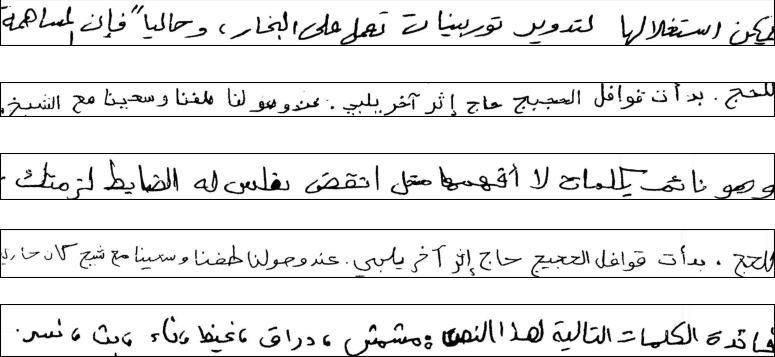
\includegraphics[width=0.9\linewidth]{Figs/fig1.png}
  \caption{Sample line images from the KHATT dataset \cite{mahmoud2014khatt}.}
  \label{fig:engagement_examples}
\end{figure}

In particular, the automated recognition and digitization of Arabic cursive handwriting present unique challenges due to the inherent complexities of the script. For one, Arabic is written from right to left, with letters assuming different shapes based on their positional context within words. In addition, diacritical marks, known as "\artext{حركات}" (harakat), and other special symbols such as the "\artext{همزة}" (hamzah) further complicate the digitization process, as many letters share identical base shapes but are distinguished by one or more dots placed above or below the character \cite{el1990arabic}. These characteristics, combined with the variability in individual handwriting styles, make the task of accurately recognizing and digitizing Arabic handwriting particularly demanding. Furthermore, because of these unique challenges, techniques developed for recognizing handwriting in other languages, such as Latin-based scripts, cannot be directly applied to Arabic, necessitating tailored approaches and specialized models \cite{alrobah2022arabic}.

Traditional Arabic HTR systems have predominantly relied on shallow learning techniques \cite{mutawa2024machine}. These methods typically involve handcrafted feature extraction processes that are sensitive to noise and degradation, limiting their effectiveness and scalability \cite{parvez2013offline}. Furthermore, most existing systems adopt a segmentation-based approach, requiring the segmentation of words into individual characters before recognition. This segmentation process is particularly challenging for Arabic due to the cursive connections between letters and the presence of similar character shapes, making it difficult to accurately isolate each character \cite{faizullah2023survey, mezghani2023recent}. In contrast, segmentation-free models (holistic approaches) recognize words as whole-word images without any segmentation processes, which can be more effective for specific applications with limited vocabularies \cite{alkhateeb2009component, nashwan2017holistic}.

Over the past decade, significant advancements in deep learning have revolutionized the field of HTR. Convolutional Neural Networks (CNNs) have emerged as the foundation of modern HTR systems due to their ability to extract complex spatial features, making them particularly effective for cursive scripts like Arabic \cite{mosbah2024adocrnet, alrobah2022arabic, altwaijry2021arabic}. Combined with Bidirectional Long Short-Term Memory (BiLSTM) networks and Connectionist Temporal Classification (CTC), deep learning models can effectively handle sequence modeling for continuous text recognition \cite{ahmad2020deep, aabed2024end, mosbah2024adocrnet,mutawa2024machine}. More recently, Transformers and attention-based models have introduced new paradigms \cite{wang2020decoupled, li2023trocr, bhunia2021metahtr}, enabling HTR systems to focus on specific regions of an image and capture long-range dependencies. These advances have significantly improved accuracy and generalizability, particularly for complex and diverse handwriting styles. Additionally, the integration of language models during post-processing has further improved prediction accuracy by leveraging contextual language information \cite{mutawa2024machine}.

To advance the development of robust HTR systems for Arabic, leveraging comprehensive and diverse datasets is paramount. While historical datasets like Muharaf \cite{saeed2024muharaf} have been valuable for analyzing historical manuscripts, there is a growing need to focus on contemporary datasets to achieve broader applicability. One such benchmark dataset is the KHATT \cite{mahmoud2012khatt,mahmoud2014khatt} dataset, which was developed by King Fahd University of Petroleum and Minerals (KFUPM) in Saudi Arabia. KHATT, an acronym for \textbf{K}FUPM \textbf{H}andwritten \textbf{A}rabic Tex\textbf{T}, also derives its name from the Arabic word (\artext{خط}), meaning ‘handwriting.’ This dataset consists of 4,000 handwritten paragraphs contributed by 1,000 writers, with each individual providing six paragraphs. The contributors reflect diverse demographics, including participants from countries such as Saudi Arabia, Morocco, the USA, Palestine, Kuwait, Egypt, Tunisia, and Yemen, representing a wide range of age groups, educational backgrounds, and both genders.

KHATT includes scanned images of handwritten text along with corresponding ground truth annotations, making it a vital resource for training and evaluating handwriting recognition systems. Its diversity in writing styles and demographics makes it especially suitable for developing generalized HTR systems that can handle the complexities of Arabic handwriting across various contexts. 


This study presents a segmentation-based HTR model utilizing advanced deep learning techniques to achieve high accuracy in Arabic handwriting recognition. The proposed system employs ResNet as a backbone for feature extraction, followed by a BiLSTM-CTC architecture for sequence modeling. To further enhance performance, a language model is incorporated during the post-processing phase, improving prediction accuracy by leveraging contextual information. In general, our contributions can be summarized as follows:


\begin{itemize}
    \item We develop a CNN-based deep learning approach combined with BiLSTM-CTC and a language model to accurately recognize Arabic handwritten text.
    % \item We design a robust preprocessing pipeline to address handwriting variability and optimize input data for recognition.
    \item We evaluate our system using the KHATT dataset, demonstrating its effectiveness across diverse handwriting styles.
\end{itemize}

The remainder of this paper is organized as follows: Section 2 provides the background, including an overview of HTR, the unique characteristics of Arabic handwriting, and essential terminology. Section 3 reviews related work, covering traditional methods, advancements in deep learning, and the importance of datasets in Arabic handwriting recognition. Section 4 outlines our methodology, detailing the proposed solution, algorithms, and techniques used to address the problem. Section 5 presents the results and evaluation, discussing the findings and their implications. Finally, Section 6 concludes the study by summarizing key contributions, addressing limitations, and proposing directions for future research.


\section{Background}
%anything here?











\subsection{Handwritten Text Recognition}

\subsubsection{Introduction to OCR and the Transition to HTR}


% Optical Character Recognition (OCR) laid the foundation for modern text recognition systems by enabling the automated extraction of text from printed documents. This field gained momentum in the 1990s \cite{parvez2013offline}, with early neural network models like LeNet \cite{lecun1998gradient} showcasing significant promise in character classification tasks. While OCR systems excelled at recognizing machine-printed text, handwritten text recognition (HTR) introduced additional complexities, such as variable writing styles, uneven spacing, and cursive connections. These challenges necessitated more advanced methodologies, evolving OCR into HTR to address the variability inherent in handwriting.


Optical Character Recognition (OCR) revolutionized text recognition by enabling the automated extraction of text from printed documents, laying the groundwork for modern systems. Early OCR systems relied heavily on accurate text localization and segmentation to isolate individual characters or lines, ensuring precise feature extraction \cite{steinherz1999comprehensive, casey1996survey}. These systems employed both micro-level features, such as character-specific edges and textures, and macro-level features, capturing broader document patterns like text alignment and spacing. Techniques such as edge-based detection (e.g., Sobel or Canny filters) \cite{canny1986computational} and statistical texture analysis quantified local properties, while keypoint descriptors like Scale-Invariant Feature Transform (SIFT) \cite{lowe2004distinctive} enhanced robustness by identifying invariant features under varying scales, rotations, or distortions.


Despite their success in recognizing machine-printed text, OCR systems faced significant challenges when applied to handwritten text. Unlike printed text, handwriting exhibits high variability in style, uneven spacing, and cursive connections, which often overlap and lack clear boundaries \cite{plamondon2000online, steinherz1999comprehensive}. These complexities demanded more sophisticated approaches that could capture the nuanced and dynamic nature of handwriting, moving beyond the rigid assumptions of traditional OCR.

The 1990s marked a pivotal era in text recognition, driven by the rise of neural network models \cite{parvez2013offline}. Innovations like LeNet \cite{lecun1998gradient} pioneered the use of convolutional layers, allowing systems to automatically learn hierarchical features directly from raw input images. This approach eliminated the reliance on handcrafted features, enabling more robust handling of variations in font styles, sizes, and distortions. With advancements in computational power, neural networks laid the groundwork for extending OCR capabilities to the more complex domain of HTR.

\subsubsection{Levels of HTR}

HTR systems tackle text recognition at different levels of granularity, beginning with character-level recognition. This approach involves recognizing isolated characters, often requiring segmentation of the text. While effective for non-cursive scripts or logographic languages like Japanese \cite{clanuwat2019kuronet} and Chinese \cite{jaderberg2015spatial}, character-level recognition struggles with cursive languages like Arabic, where the shapes of letters depend on their position and surrounding context.

To overcome these limitations, word-level recognition transcribes individual handwritten words as single units, reducing the dependency on character segmentation and improving accuracy for cursive scripts \cite{bhunia2019handwriting}. More advanced techniques have focused on line-level recognition, where entire lines of text, including spaces, are transcribed. Line-level HTR can either rely on pre-segmented input or integrate segmentation and recognition into a unified framework. Line-level recognition introduces challenges related to spatial and contextual coherence, as the relationships between words and characters must be preserved. However, it offers a balance between complexity and efficiency, making it particularly relevant for cursive scripts like Arabic.

In recent developments, systems also tackle paragraph- and page-level recognition, incorporating layout analysis for handling complex document structures. These approaches combine transcription with spatial segmentation tasks, allowing models to process structured documents and extract meaningful text from diverse layouts \cite{such2018fully, bhunia2019handwriting}. As the levels progress from character to page, the complexity increases, requiring more robust handling of spatial and contextual relationships.

\subsubsection{Sequential Nature of Handwriting}

Handwriting is inherently sequential, with characters and words influenced by their position and surrounding context within a sequence. Recognizing handwriting requires models capable of capturing these dependencies to ensure accurate transcription. Rcurrent neural networks (RNNs), introduced in \cite{rumelhart1986learning}, are particularly well-suited for this task. Their feedback loops enable information to persist across time steps, allowing them to model sequential dependencies effectively. This capability makes RNNs a natural choice for handwriting recognition, where the relationship between characters is critical.

Despite their advantages, standard RNNs face significant challenges in handling long sequences due to the vanishing gradient problem \cite{bengio1994learning}. During training, the backpropagation algorithm calculates gradients to adjust network weights. In RNNs, gradients are propagated through time steps by repeated multiplication. Over long sequences, these gradients tend to shrink exponentially, often becoming too small to update the weights effectively. This issue is exacerbated by activation functions such as sigmoid or tanh, which compress their outputs into a narrow range, further diminishing the gradients.

For that, long short-term memory (LSTM) networks, introduced in \cite{hochreiter1997long}, were specifically designed to overcome the vanishing gradient problem. LSTMs introduce memory cells and gating mechanisms (input, forget, and output gates) that regulate the flow of information through the network. These mechanisms enable LSTMs to selectively retain or discard information, allowing them to maintain long-term dependencies. For example, in handwriting recognition, an LSTM can retain information about a diacritical mark, like "\artext{ضمّة}" (damma), at the beginning of a word while processing subsequent characters, ensuring accurate transcription within context.

Bidirectional LSTMs (BiLSTMs), introduced in \cite{schuster1997bidirectional}, extend the LSTM architecture by processing sequences in both forward and backward directions. This bidirectional processing allows the model to consider both preceding and succeeding context, making it particularly effective for cursive handwriting, where the interpretation of a character often depends on its neighbors.

For tasks involving 2D input data, such as handwritten line images, Multidimensional LSTM (MDLSTM) networks, introduced in \cite{graves2007multi}, further enhance sequential modeling by introducing recurrence along two spatial dimensions. This architecture captures dependencies in both horizontal and vertical directions, making it ideal for processing handwritten text. However, the computational demands of MDLSTMs have led to a shift toward hybrid models that combine Convolutional Neural Networks (CNNs) for spatial feature extraction with BiLSTMs for sequence modeling. These hybrid architectures balance accuracy and efficiency, forming the backbone of modern handwriting recognition systems.



\subsubsection{CTC Loss and Decoding}



A key component in modern HTR systems is the use of Connectionist Temporal Classification (CTC) as a loss function and decoding mechanism. Introduced by Graves et al. \cite{graves2006connectionist}, CTC enables sequence-to-sequence learning when the input (e.g., image features) and output (e.g., character sequences) lengths differ. It allows models to align variable-length inputs and outputs without requiring pre-segmented data, a significant challenge in HTR.

CTC introduces a special "blank" token ("\(- \)") to handle gaps in alignment, letting the model represent transitions between characters or accommodate uneven spacing and cursive connections. This design is ideal for HTR, where the input sequence often exceeds the target transcription in length and characters may not align neatly to time steps.

CTC computes the conditional probability of a target transcription \( l \) given the model’s output \( Y \), which consists of \( T \) time steps. Each step \( y_t \) is a probability distribution over all possible characters, including the blank token. The conditional probability \( p(l|Y) \) is defined in Equation~\ref{eq:ctc-prob} as:

\begin{equation}
  p(l|Y) = \sum_{\pi : M(\pi) = l} p(\pi|Y), 
  \label{eq:ctc-prob}
  \end{equation}

where \( \pi \) represents all possible alignments of \( Y \) that map to \( l \), and \( M(\pi) \) removes repeated characters and blanks from \( \pi \). For example, "\( -- \)\artext{للل}\(--\)\artext{اااا}\( -- \)\artext{ث}--\artext{مم}-" gets aligned to the target "\artext{مثال}". The sequence output is the probability of \( \pi \) at time step \( t \), which is defined in Equation~\ref{eq:alignment-prob} as:


\begin{equation}
  p(\pi|Y) = \prod_{t=1}^T y^{t}_{\pi_t}, 
  \label{eq:alignment-prob}
  \end{equation}

where \( y^{t}_{\pi_t} \) is the output probability of the character \( \pi_t \) at time step \( t \), as described in \cite{shi2016endtoend}. This formula accounts for the cumulative probability of the alignment \( \pi \) across all time steps.


The CTC loss function, shown in Equation~\ref{eq:ctc-loss}, sums over all possible alignments \( \pi \) that produce the target sequence \( l \). It is efficiently computed using a dynamic programming approach, which calculates the forward and backward paths:

\begin{equation}
  \mathcal{L}_{CTC} = -\log \sum_{\pi : M(\pi) = l} \prod_{t=1}^T y^{t}_{\pi_t}.
  \label{eq:ctc-loss}
  \end{equation}

Furthermore, CTC decoding converts the probabilistic output \( Y \) into a transcription through two main strategies: (1) greedy decoding and (2) beam search decoding. On the one hand, greedy decoding selects the character with the highest probability at each time step. While fast and computationally efficient \cite{graves2006connectionist}, it often ignores global dependencies, leading to suboptimal results in complex handwriting or ambiguous cases. On the other hand, beam search decoding improves accuracy by maintaining multiple candidate transcriptions (the "beam") and evaluating their overall probabilities. This method captures context more effectively and is particularly advantageous for cursive or highly variable handwriting, as highlighted in \cite{praneetha2023handwritten, shi2016endtoend}.


CTC transforms HTR by allowing models to learn temporal alignments directly from data, avoiding the need for explicit segmentation. 

\subsubsection{Deep Learning Advancements in HTR}

Recent advancements in deep learning, particularly attention-based models and transformers, have revolutionized HTR. Unlike RNNs, which process sequences step by step, transformers analyze an entire input sequence simultaneously, capturing long-range dependencies while dynamically focusing on specific regions of the input image. This architecture, introduced in \cite{vaswani2017attention}, has fundamentally changed how sequential data is processed in deep learning.

A helpful analogy is how humans read text. Instead of scanning every letter in a linear fashion, we focus more on unclear or important areas while using surrounding context to fill in gaps. Similarly, transformers use attention mechanisms to emphasize ambiguous or complex sections of handwriting while retaining global context. For example, if a character in the word "\artext{مثال}" (example) is unclear, the transformer can reference the rest of the word to infer its correct identity.

This dynamic attention mechanism enables modern HTR systems to excel with diverse handwriting styles, from cursive to decorative scripts, by adapting to stylistic variations and spatial irregularities. Transformers’ ability to process sequences holistically has set new benchmarks in accuracy and generalizability, making them integral to state-of-the-art HTR systems.


\subsection{Characteristics of Arabic Handwriting}

Arabic handwriting possesses several distinctive features that present unique challenges for Handwritten Text Recognition (HTR) systems. A comprehensive understanding of these characteristics is essential for developing effective recognition models tailored to the intricacies of the Arabic script. This section delineates the primary attributes of Arabic handwriting that influence the design and performance of HTR systems.

\subsubsection{Character Level Characteristics}

The Arabic alphabet comprises 28 primary characters, each of which does not have distinct uppercase or lowercase forms. Instead, each character can adopt two to four different shapes depending on its position within a word: isolated, initial, medial, or final \cite{alrobah2022arabic}. Consequently, the 28 Arabic letters are represented by 84 distinct forms. Table~\ref{table:arabic_characters} illustrates the Arabic letters in their four positional forms, detailing the letter order in the Arabic alphabet, pronunciation, and the various shapes each letter assumes based on its placement within a word. Notably, separating characters, such as "\artext{ا}" (Alif) and "\artext{ر}" (Raa), have only two forms: isolated and final.

\begin{table*}[ht]
  \renewcommand{\arraystretch}{1.5}
  \caption{Arabic Characters in the 4 Forms: Isolated, Beginning, Middle, and End}
  \label{table:arabic_characters}
  \centering
  \begin{tabular}{|c|c|c|c|c|c|c|c|c|c|c|c|}
  \hline
  \textbf{No.} & \textbf{Pronunciation} & \textbf{Isolated} & \textbf{Beginning} & \textbf{Middle} & \textbf{End} & \textbf{No.} & \textbf{Pronunciation} & \textbf{Isolated} & \textbf{Beginning} & \textbf{Middle} & \textbf{End} \\
  \hline
  1  & Alef & \artext{ا} & \artext{ا} & \artext{ا} & \artext{ـا} & 15 & Dhad  & \artext{ض} & \artext{ضـ} & \artext{ـضـ} & \artext{ـض} \\
  2  & Baa  & \artext{ب} & \artext{بـ} & \artext{ـبـ} & \artext{ـب} & 16 & Taa   & \artext{ط} & \artext{طـ} & \artext{ـطـ} & \artext{ـط} \\
  3  & Taa  & \artext{ت} & \artext{تـ} & \artext{ـتـ} & \artext{ـت} & 17 & Thaa  & \artext{ظ} & \artext{ظـ} & \artext{ـظـ} & \artext{ـظ} \\
  4  & Thaa & \artext{ث} & \artext{ثـ} & \artext{ـثـ} & \artext{ـث} & 18 & Ain   & \artext{ع} & \artext{عـ} & \artext{ـعـ} & \artext{ـع} \\
  5  & Jeem & \artext{ج} & \artext{جـ} & \artext{ـجـ} & \artext{ـج} & 19 & Ghain & \artext{غ} & \artext{غـ} & \artext{ـغـ} & \artext{ـغ} \\
  6  & Haa  & \artext{ح} & \artext{حـ} & \artext{ـحـ} & \artext{ـح} & 20 & Faa   & \artext{ف} & \artext{فـ} & \artext{ـفـ} & \artext{ـف} \\
  7  & Khaa & \artext{خ} & \artext{خـ} & \artext{ـخـ} & \artext{ـخ} & 21 & Qaf   & \artext{ق} & \artext{قـ} & \artext{ـقـ} & \artext{ـق} \\
  8  & Dal  & \artext{د} & \artext{د}  & \artext{د}  & \artext{ـد} & 22 & Kaf   & \artext{ك} & \artext{كـ} & \artext{ـكـ} & \artext{ـك} \\
  9  & Thal & \artext{ذ} & \artext{ذ}  & \artext{ذ}  & \artext{ـذ} & 23 & Lam   & \artext{ل} & \artext{لـ} & \artext{ـلـ} & \artext{ـل} \\
  10 & Raa  & \artext{ر} & \artext{ر}  & \artext{ر}  & \artext{ـر} & 24 & Meem  & \artext{م} & \artext{مـ} & \artext{ـمـ} & \artext{ـم} \\
  11 & Zai  & \artext{ز} & \artext{ز}  & \artext{ز}  & \artext{ـز} & 25 & Noon  & \artext{ن} & \artext{نـ} & \artext{ـنـ} & \artext{ـن} \\
  12 & Seen & \artext{س} & \artext{سـ} & \artext{ـسـ} & \artext{ـس} & 26 & Ha    & \artext{ه} & \artext{هـ} & \artext{ـهـ} & \artext{ـه} \\
  13 & Sheen& \artext{ش} & \artext{شـ} & \artext{ـشـ} & \artext{ـش} & 27 & Waw   & \artext{و} & \artext{و}  & \artext{و}  & \artext{ـو} \\
  14 & Sad  & \artext{ص} & \artext{صـ} & \artext{ـصـ} & \artext{ـص} & 28 & Yaa   & \artext{ي} & \artext{يـ} & \artext{ـيـ} & \artext{ـي} \\
  \hline
  \end{tabular}
  \end{table*}

\subsubsection{Diacritical Marks (Dots)}
Dots are integral components of Arabic letters, playing a crucial role in distinguishing characters that share the same primary strokes. Arabic utilizes 16 main strokes, and the presence, absence, or placement of dots can differentiate between letters with identical base shapes. For instance, the letters "\artext{ب}" (Ba), "\artext{ت}" (Ta), and "\artext{ث}" (Tha) are differentiated solely by the number and position of dots below them. Accurate recognition of these diacritical marks is essential to prevent misclassification and ensure the correct interpretation of words. Table~\ref{table:main_strokes} shows the 16 main strokes of the Arabic script, and able~\ref{table:characters_with_dots} displays the letters categorized by one, two, or three dots.


\begin{table}[ht]
\renewcommand{\arraystretch}{1.3}
\caption{Main Arabic Characters Strokes}
\label{table:main_strokes}
\centering
\begin{tabular}{|c|}
\hline
\textbf{Arabic Main Stroke} \\
\hline
\rule{0pt}{10pt} \artext{ا ب ج د ر س ص ط ع ف ك ل م ن و ي} \rule[-8pt]{0pt}{8pt} \\ % Equal padding
\hline
\end{tabular}
\end{table}

\begin{table}[ht]
  \renewcommand{\arraystretch}{1.3}
  \caption{Arabic Characters That Have One, Two, or Three Dots}
  \label{table:characters_with_dots}
  \centering
  \begin{tabular}{|c|>{\centering\arraybackslash}p{6cm}|}
  \hline
  \textbf{No. of Dots} & \textbf{Letters} \\
  \hline
  \rule{0pt}{10pt} One dot   & \artext{ب ج خ ذ ز ض ظ غ ف ن} \rule[-8pt]{0pt}{8pt} \\ % Equal padding for row
  \hline
  \rule{0pt}{10pt} Two dots  & \artext{ت ق ي} \rule[-8pt]{0pt}{8pt} \\ % Equal padding for row
  \hline
  \rule{0pt}{10pt} Three dots & \artext{ث ش} \rule[-8pt]{0pt}{8pt} \\ % Equal padding for row
  \hline
  \end{tabular}
\end{table}

\subsubsection{Hamzah: A Special Character}

The hamzah "\artext{ء}" is a unique character in the Arabic script that can function as a primary character or as a subcomponent integrated within other primary characters \cite{ahmed2020offline}. For example, the hamzah appears as a standalone character in words like "\artext{سماء}" (samā’, meaning sky) and "\artext{هواء}" (hawā’, meaning air). Additionally, the hamzah can be incorporated within other letters, such as "\artext{ك}", "\artext{أ}", "\artext{ئ}", "\artext{ؤ}", and "\artext{إ}". Moreover, the placement of the hamzah, whether above, below, or within a letter, determines its pronunciation and role within different word contexts.

\subsubsection{ Diacritics: Tashkeel and Tanween}

"\artext{التشكيل}" (tashkeel), also known as "\artext{حركات}" (harakat), and "\artext{التنوين}" (tanween) are diacritical marks used in Arabic to indicate pronunciation and grammatical nuances \cite{eltay2020exploring}.  Tashkeel consists of five symbols that modify the meaning and pronunciation of words. For example, the words "\artext{عِلْم}" (ilm, meaning knowledge) and "\artext{عَلَم}" (alam, meaning flag) share the same base characters but differ in their Tashkeel, altering their meanings significantly. Although Tashkeel is not extensively used in everyday Arabic writing, since context often clarifies meaning, it is essential for novice readers and in educational materials. Tashkeel can change the semantic interpretation of words, making its accurate recognition (if present) vital for preserving textual integrity.

\subsubsection{Cursive Nature and Baseline Structure}
Arabic is inherently a cursive script in both its printed and handwritten forms, meaning that letters within words are connected by a horizontal line known as the baseline \cite{alrobah2022arabic}. Portions of characters that extend below the baseline are referred to as "descenders," while those that extend above are termed "ascenders." Figure~\ref{fig:ab} depicts the baseline with ascenders and descenders, highlighting how these elements contribute to the overall structure and flow of Arabic handwriting. This cursive connectivity facilitates fluid writing but complicates the recognition process, as it introduces variability in letter shapes and spacing.

\begin{figure}[ht]
  \centering
  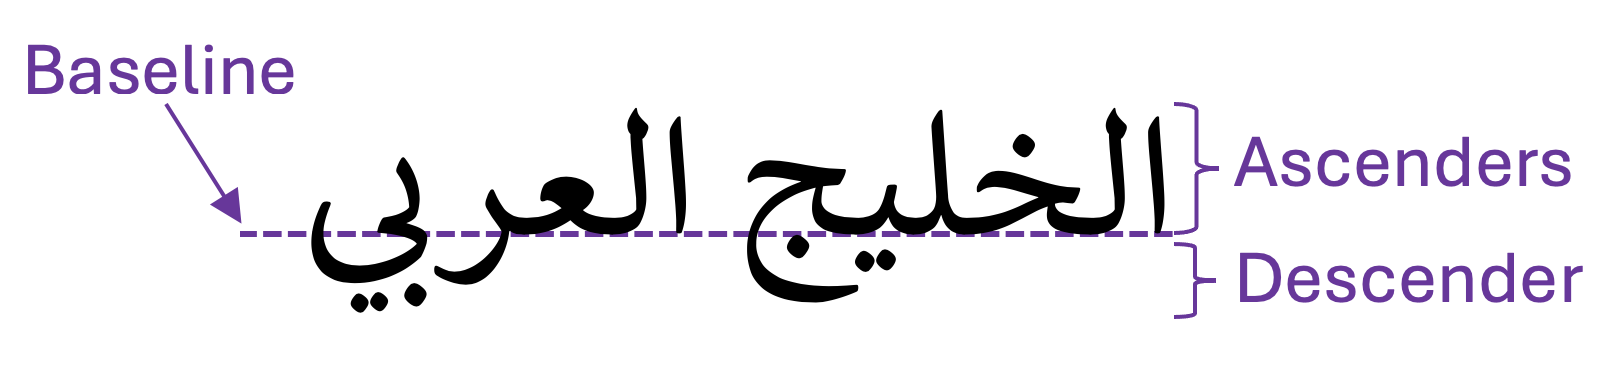
\includegraphics[width=0.8\linewidth]{Figs/fig2.png}
  \caption{Illustration of the baseline, ascenders, and descenders in the Arabic phrase "\artext{الخليج العربي}" (The Arabian Gulf).}
  \label{fig:ab}
\end{figure}

\subsubsection{Separating Characters and Word Segmentation}

Arabic includes six separating characters namely 
"\artext{ا}", "\artext{ر}", "\artext{ز}", "\artext{د}", "\artext{ذ}" and "\artext{و}", which are not connected to the characters that follow them \cite{alrobah2022arabic}. These separating characters divide words into smaller units known as Parts of Arabic Words (PAWs). Each word may consist of one or more PAWs depending on the presence of separating characters. Accurate segmentation of PAWs is critical for effective HTR, as it influences the ability to isolate and recognize individual characters within connected scripts. Examples of words composed of one, two, three, four, or five PAWs are presented in Table~\ref{table:words_with_paws}.

\begin{table}[ht]
  \renewcommand{\arraystretch}{1.3}
  \caption{Examples of Words with One, Two, Three, Four, and Five PAWs}
  \label{table:words_with_paws}
  \centering
  \begin{tabular}{|c|>{\centering\arraybackslash}p{2cm}|>{\centering\arraybackslash}p{3cm}|}
  \hline
  \textbf{No. of PAWs} & \textbf{Example} & \textbf{Division (Right-to-Left)} \\
  \hline
  \rule{0pt}{10pt} One PAW   & \artext{ليث}       & \artext{ليث} \rule[-8pt]{0pt}{8pt} \\ 
  \hline
  \rule{0pt}{10pt} Two PAWs  & \artext{حمزة}      & \artext{حمز  + ة} \rule[-8pt]{0pt}{8pt} \\ 
  \hline
  \rule{0pt}{10pt} Three PAWs & \artext{إبراهيم}  & \artext{إ + برا + هيم} \rule[-8pt]{0pt}{8pt} \\ 
  \hline
  \rule{0pt}{10pt} Four PAWs  & \artext{نورة}     & \artext{نو + رة} \rule[-8pt]{0pt}{8pt} \\ 
  \hline
  \rule{0pt}{10pt} Five PAWs  & \artext{أوراد}    & \artext{أ + و + را + د} \rule[-8pt]{0pt}{8pt} \\ 
  \hline
  \end{tabular}
\end{table}




\subsubsection{Overlapping in Handwritten PAWs}
In handwritten Arabic, PAWs may exhibit vertical overlapping, where characters within a word or between adjacent words overlap vertically. Figure ~\ref{fig:vo} illustrates examples of such overlapping, demonstrating how characters can intertwine, making segmentation and recognition more challenging. This overlapping is a common occurrence in cursive handwriting and requires robust HTR systems capable of accurately distinguishing and recognizing characters despite such distortions.

\begin{figure}[ht]
  \centering
  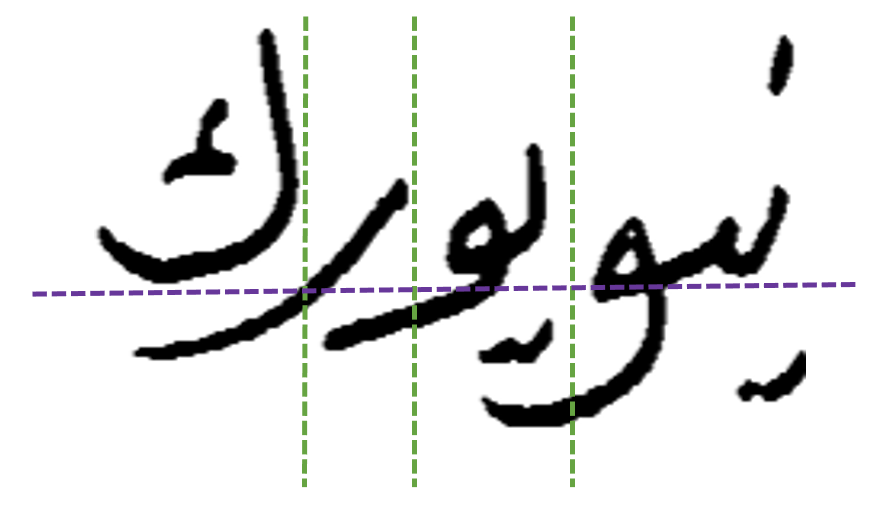
\includegraphics[width=0.7\linewidth]{Figs/fig3.png}
  \caption{Vertical overlapping between two PAWs occurring twice within the same handwritten word.}
  \label{fig:vo}
\end{figure}


\subsection{Challenges in Arabic HTR}

The recognition of Arabic handwritten text poses unique challenges due to the intricacies of the script, the variability of its handwritten forms, and the limitations of current resources and methodologies. This section explores these challenges in depth, highlighting the inherent difficulties that hinder the development of robust Arabic HTR systems.


\subsubsection{High Variability in Handwriting Styles}

Arabic handwriting exhibits a significant degree of variability, making it one of the most challenging scripts to process \cite{kasem2023advancements}. Unlike many other scripts, Arabic handwriting allows for a broad range of stylistic diversity that is still considered acceptable. Individual differences in stroke thickness, letter spacing, slant, and elongation further contribute to the variation in handwritten forms. These stylistic differences are not arbitrary; they are often influenced by cultural and regional preferences. For example, traditional calligraphic styles such as "\artext{النسخ}" (Naskh), "\artext{الرقعة}" (Ruq’ah), and "\artext{الكوفي}" (Kufi) have distinct proportions and connections, which can manifest even in casual handwriting. Figure ~\ref{fig:mr}  illustrates examples of handwritten Arabic, showcasing the variability across different writers and styles.


\begin{figure}[ht]
  \centering
  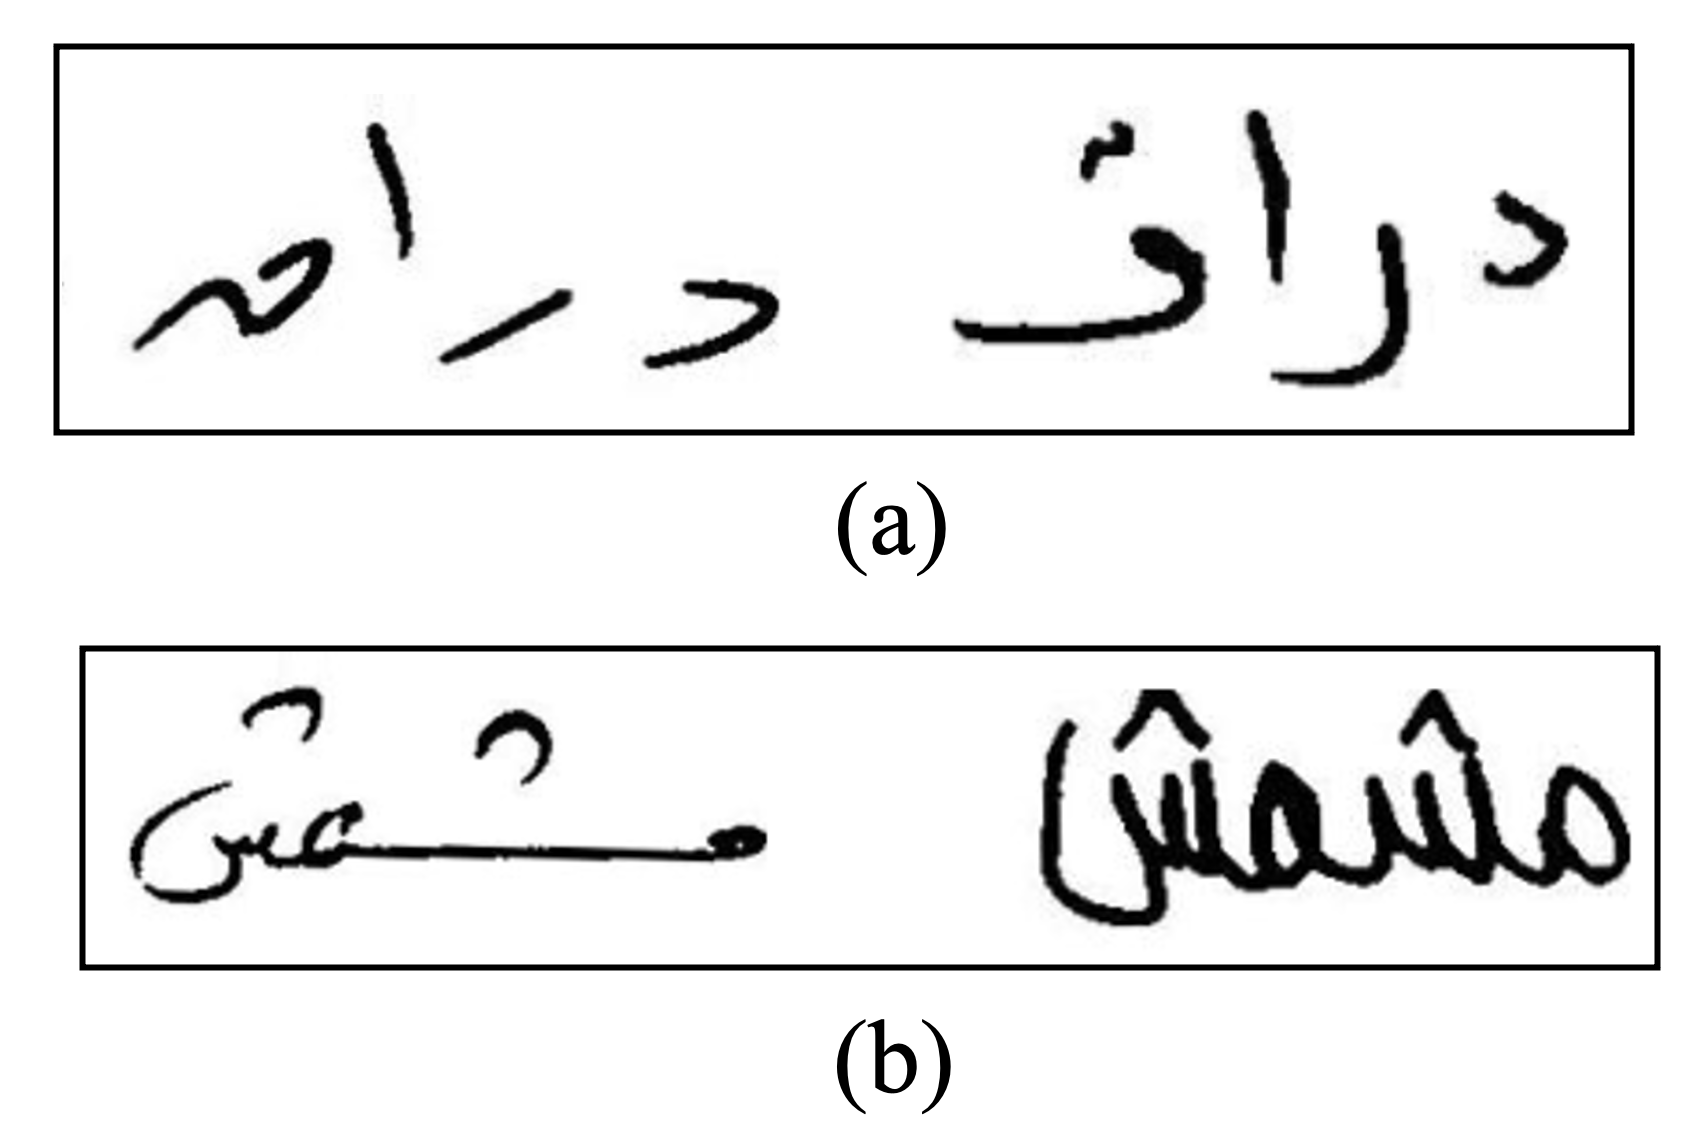
\includegraphics[width=0.7\linewidth]{Figs/fig4.png}
  \caption{Handwritten Arabic words from the KHATT dataset: (a) \artext{دراق} (Duraq, 'plum') and (b) \artext{مشمش} (Mishmish, 'apricot'), showcasing variability in letters like \artext{ش}, \artext{م}, \artext{د}, \artext{ر}, and \artext{ق} across writers.}
  \label{fig:mr}
\end{figure}

Additionally, Arabic handwriting is not restricted to a single standardized form. Variants of Modern Standard Arabic (MSA) often appear in handwritten texts, including informal adaptations and regional orthographic practices. Although HTR systems are not tasked with interpreting dialects or regional meanings, the visual form of these handwritten variants, such as alternative spellings or elongated structures, introduces challenges in character recognition. This vast variability complicates segmentation and encoding, where traditional OCR systems fail due to their reliance on rigid, rule-based approaches. Unlike scripts with default spaces between characters, Arabic’s cursive nature creates continuous connections between letters, making segmentation into discrete units a formidable task. \\


\subsubsection{Right-to-Left Directionality and Structural Bias}


The right-to-left (RTL) directionality of Arabic script presents significant challenges for handwritten text recognition (HTR) systems, which are predominantly designed for left-to-right (LTR) languages \cite{abdulmuttalib2021rtl}. This fundamental difference impacts multiple aspects of HTR, including preprocessing, feature extraction, and sequence modeling, necessitating specific adaptations to ensure effective processing of Arabic text.


Arabic text flows from the top-right to the left, a structure that conflicts with the design assumptions underlying most LTR-oriented algorithms. This discrepancy is especially evident in preprocessing tasks, such as baseline detection and text alignment. In Arabic handwriting, the baseline is often influenced by interactions between ascenders (e.g., "\artext{ط}") and descenders (e.g., "\artext{ي}"), which are more prominent in cursive styles. Traditional baseline detection methods, typically designed for LTR languages, often fail to account for these interactions, leading to errors in segmentation and recognition \cite{khattab2019arabic}. Such misalignments not only distort spatial positioning but also propagate errors through subsequent processing stages.


Convolutional Neural Networks (CNNs), widely used in modern HTR systems, exacerbate these challenges due to their sliding window mechanism. CNNs extract features by moving a kernel across an image from left to right \cite{lecun1998gradient}. While this design is effective for LTR scripts, it introduces a structural bias when applied to Arabic handwriting. In this case, the CNN begins processing at the visual end of a word and progresses toward its beginning, disrupting the natural contextual flow. This misalignment particularly affects connected letters and diacritics, both of which are critical for accurate recognition of Arabic text.

One common workaround is to horizontally flip the input image, effectively reversing the text flow to make it appear left-to-right \cite{saeed2024muharaf, chan2024hatformer}. While this approach enables LTR-designed systems to process Arabic text more effectively, it introduces its own set of problems. Flipping the text can distort spatial relationships, particularly for overlapping characters or diacritics, and fails to address the inherent architectural bias in the CNN. Although flipped input aligns the image for feature extraction, it does not resolve sequence alignment issues during decoding, where the reversed order can still affect performance.

Sequence modeling architectures, such as RNNs and transformers, encounter additional challenges with RTL directionality. RNNs process sequences step-by-step, making them sensitive to the order of input data. When trained on LTR sequences, an RNN processes Arabic text in reverse, beginning at the end of a word or sentence and losing the natural semantic flow required for contextual understanding \cite{chan2024hatformer}. Although transformers are more flexible due to their self-attention mechanisms, they face similar problems. Positional encodings in pretrained transformer models are typically designed for LTR scripts. Applying these encodings to Arabic text misaligns attention distributions, reducing the model’s ability to accurately focus on the initial characters in a sequence.


\section{Related Work}
In this section, we review previous research on Arabic HTR, focusing on the development and utilization of Arabic handwriting datasets, preprocessing techniques, and advancements in deep learning methodologies that have significantly advanced the field.

\subsection{Datasets of Arabic Handwriting}

Several datasets have been developed to facilitate Arabic handwriting research, each varying in focus, size, and availability. Below, we summarize the most relevant datasets, including KHATT, IFN/ENIT, MADCAT, AHDB, and Muharaf.



% \begin{itemize}
  
%     \item \textbf{KHATT Dataset \cite{mahmoud2014khatt}:} \\ 
%     The KHATT dataset is a modern Arabic handwriting dataset comprising 4,000 paragraphs written by 1,000 scribes, with six paragraphs contributed by each.  was developed jointly by researchers from KFUPM (Saudi Arabia), TU Dortmund (Germany), and TU Braunschweig (Germany). 

%     KHATT is an offline Arabic handwritten dataset.
%     collection of 1000 forms, 2000 (random and fixed paragraphs) & free paragraphsfrom 46 different sources. Each form consists of 4 pages. The first page contains writer information. The second and third pages contain a fixed text paragraph and a free text paragraph respectively. Finally, on the fourth page open and free text is written on a ruled baseline to avoid skew ... each writer had to write four paragraphs: the first is a paragraph that covers all the shapes of Arabic letters, and the writer had to write it twice; the second is a paragraph that is extracted from different forms, the third is free writing paragraph. A total of 2000 paragraphs were extracted



%     \item \textbf{IFN/ENIT Dataser \cite{mahmoud2014khatt}:} \\
%     is probably the most widely used and cited database [10,11].
%     Database is a Handwritten Arabic dataset of Tunisian town/village names that are developed by the Institute for Communications Technology (IFN) and Ecole Nationale d’Ingénieur de Tunis (ENIT). Four hundred eleven different writers participated in filling 2,265 forms of selected names from a collection of 946 Tunisian town/village names with the postcode. The forms were scanned, and the words with the ground truth data were extracted automatically, and the writers’ information is also added. Then these data were verified manually. Each name may consist of more than one word with a total of 26,459 handwritten words and 115,585 PAWs (Part of Arabic Words).


%     \item \textbf{Muharaf Dataset \cite{saeed2024muharaf}:} \\
%     The Muharaf dataset, used in this study, is the largest publicly available Arabic dataset with fully annotated and transcribed historical manuscripts at the text-line level. It includes 1,644 pages (1,216 public and 428 restricted), spanning the early 19th to the early 21st century, with 36,311 text lines (24,495 public). Line-level images, stored in PNG format, were generated using line warping software to create consistent horizontal grids, and extensive metadata is provided in JSON format.


%     MADCAT (Multilingual Automatic Document Classification Analysis and Translation) is a five year technology evaluation program sponsored by the US Defense Advanced Research Projects Agency (DARPA), with main focus on machine translation, produced in its first phase a Training Set of Arabic handwritten text [13]. This data is created by the Linguistic Data Consortium (LDC) to support Phase 1 of the DARPA MADCAT Program. The dataset comprises 9693 collected handwritten pages, original Arabic source documents (tokenized and sentence-segmented); scanned images at 600 dpi of the corresponding handwritten page for each document; ground truth annotations for each handwritten page; and English translations for each document. The data sources are news groups, newswire and weblogs. The dataset is not freely available to non-members and scanned at 600 dpi resolution only.However, this dataset is not freely available to the public, which restricts its use.


%     AHDB [53] is an Arabic Handwritten words dataset developed by Al-ma’adeed et al. it consists of Arabic handwritten words and free Arabic handwritten sentences and pages. They searched for the top 20 common words in Arabic. They designed a Six-page form with 96 words of the common 20 Arabic words and the literal amounts used in cheques. The word and writer’s identification numbers are saved with every image.

%     \item \textbf{Muharaf Dataset \cite{saeed2024muharaf}:} \\
%     The Muharaf dataset is the largest publicly available Arabic dataset with fully annotated and transcribed historical manuscripts at the text-line level. It includes 1,644 pages (1,216 public and 428 restricted), spanning the early 19th to the early 21st century, with 36,311 text lines (24,495 public). Line-level images, stored in PNG format, were generated using line warping software to create consistent horizontal grids, and extensive metadata (incl. griundtruth) is provided in JSON format.
  
% \end{itemize}

\begin{itemize}
  \item \textbf{KHATT Dataset \cite{mahmoud2012khatt, mahmoud2014khatt}:} \\
  The KHATT dataset, used in this study, is a modern Arabic handwriting dataset comprising 4,000 paragraphs written by 1,000 scribes, with each scribe contributing four paragraphs. Developed jointly by researchers from KFUPM in Saudi Arabia, Technische Universität Dortmund (TU Dortmund), and Technische Universität Braunschweig (TU Braunschweig) in Germany, KHATT provides a comprehensive resource for training and evaluating HTR systems. The dataset includes 1,000 forms, each containing four pages: the first page holds writer information, the second and third pages feature fixed and free text paragraphs respectively, and the fourth page contains open and free text written on a ruled baseline to minimize skew. This structure ensures consistency and facilitates the extraction of 2,000 randomly selected and fixed paragraphs from 46 different sources.

  \item \textbf{IFN/ENIT Dataset \cite{pechwitz2002ifn}:} \\
  The IFN/ENIT dataset is one of the most widely used and cited Arabic handwritten databases. Developed by the Institute for Communications Technology (IFN) and Ecole Nationale d’Ingénieur de Tunis (ENIT) in Tunisia, this dataset consists of handwritten Tunisian town and village names. It includes 2,265 forms filled out by 411 different writers, covering 946 Tunisian town and village names along with their postcodes. Each form is scanned, and the handwritten words are automatically extracted and annotated with ground truth data, which is then manually verified. The dataset encompasses 26,459 handwritten words and 115,585 PAWs, making it a valuable resource for evaluating HTR systems' performance in recognizing geographically specific Arabic text.

  \item \textbf{MADCAT Dataset \cite{lee2012madcat}:} \\
  The MADCAT (Multilingual Automatic Document Classification, Analysis, and Translation) dataset is part of a five-year technology evaluation program sponsored by the US Defense Advanced Research Projects Agency (DARPA). Created by the Linguistic Data Consortium (LDC), MADCAT focuses on machine translation and includes a training set of Arabic handwritten text. The dataset comprises 9,693 handwritten pages, each accompanied by scanned images, tokenized and sentence-segmented original Arabic source documents, ground truth annotations, and English translations. The data sources include newsgroups, newswire, and weblogs. However, MADCAT is not freely available to the public, restricting its use to members and participants of the DARPA program.

  \item \textbf{AHDB Dataset \cite{al2002data}:} \\
  The Arabic Handwritten Database (AHDB) consists of Arabic handwritten words, free handwritten sentences, and pages. The dataset includes the top 20 most common Arabic words, collected through a six-page form containing 96 instances of these words and their literal amounts used in cheques. Each image is annotated with the corresponding word and writer identification numbers. AHDB provides a diverse set of handwriting samples, aiding in the training of deep learning-based HTR models capable of handling both isolated words and connected text.

  \item \textbf{Muharaf Dataset \cite{saeed2024muharaf}:} \\
  The Muharaf dataset is the largest publicly available Arabic dataset with fully annotated and transcribed historical manuscripts at the text-line level. It encompasses 1,644 pages (1,216 public and 428 restricted), spanning from the early 19th to the early 21st century, and includes 36,311 text lines (24,495 public). Line-level images are stored in PNG format and were generated using line warping software to create consistent horizontal grids. Extensive metadata, including ground truth annotations, is provided in JSON format. This dataset is instrumental for training and evaluating HTR systems aimed at digitizing and preserving historical Arabic literature, addressing challenges related to noise, degradation, and archaic handwriting styles.
\end{itemize}





\subsection{Preprocessing Techniques}

Preprocessing techniques are a crucial pre-requisite to any model's input. It ensures that the model is able to focus on the important features of the input to enable it to better detect patterns. In our case, our input is images that are handwritten Arabic documents and so it is crucial to ensure that the models are receiving input that can allow it to identify handwriting, letter styles, and strokes. 

A means of doing this is binarization. Binarization is a crucial preprocessing step that transfroms input images, whether they are RGB or grayscale, into a simplified binary format. The purpose of this is to highlight character strokes and remove unneccessary image color information. There are different ways to apply thresholds for binarization, the most prominent being global thresholding where beyond a certain threshold, the pixel is set to 1 and below that, set to 0. A more robust way is Otsu's method \cite{otsu1979aa} that finds an optimal global threshold by minimizing intra-class variance. It has been also proven to exhibit lower running times at a mean of 2 seconds \cite{sahlol2014proposed}. Another approach is differentiable binarization that integrates the binarization process into network training, allowing it to be part of optimization and loss calculations \cite{liao2022real}. Differentiable binarization uses an adaptive threshold map learned from the network to apply different thresholds on different parts of the image which is useful in areas of low confidence in boundary regions compared to areas of high confidence centrally within the image. Furthermore, this layer can be removed once the model is trained to ensure that inference time is not impacted.  

Another measure of preprocessing is noise removal. Noise removal is a crucial step as images often do not come in ideal conditions leading to poor model performance if fed directly. One of the techniques of noise removal is median filtering. The median of a group of pixels (3x3, 5x5, 7x7, etc.) that surround a specific pixel (its neighborhood) replaces the pixel to smooth out and reduce noise within the image \cite{sahlol2014proposed,alghyaline2023arabic}. Another common category of techniques is morphological operations. These operations manipulate the shape of the input images. These operations include dilation, erosion, opening, and closing \cite{alghyaline2023arabic}. Dilation adds pixels to the boundaries of objects in an image making them thicker within the image. Conversely, erosion removes pixels from object boundaries, eliminating pixels that are isolated. Opening and closing are then combinations of erosion and dilation that help find the right balance between refining object shapes and eliminating noise. 




\subsection{Deep Learning Approaches for HTR}

Many HTR systems have been developed to recognize Arabic handwritten characters and words. CNNs have been widely employed in handwritten recognition due to their capacity to autonomously acquire hierarchical features from raw pixel inputs \cite{}.

There have been multiple variations of CNNs developed to tackle a number of datasets pertaining to Arabic handwritten text. An example of this is a simple CNN trained on the Arabic Handwritten Characters Dataset (AHCD) that used two convolutional, two pooling, and two fully connected layers \cite{el2017arabic}. This architecture was able to gain an accuracy of 94.9\% which is overall good but might be attributed to the dataset and its characteristics. Similar models were run on different datasets such as Hijja \cite{altwaijry2021arabic} that got a lower accuracy of 88\% but improved results on AHCD (97\%). The addition of batch normalization and dropout layers only slightly improved performance on AHCD getting an accuracy of 97.6\% \cite{younis2017arabic}. Adding more convolutional layers (four) only increases the initial accuracy to 97.2\% \cite{najadat2019arabic}. 


Another common approach involves combining CNNs with other classifiers, such as Support Vector Machines (SVMs), to enhance recognition accuracy. For instance, Elleuch et al. \cite{elleuch2016new} utilized a combination of CNN and SVM with dropout regularization to recognize offline Arabic handwritten characters, achieving error classification rates of 5.83\% on the Handwritten Arabic Characters Database (HACDB) and 7.05\% on the IFN/ENIT dataset.

RNNs, particularly BiLSTM networks, have also been integrated with CNNs to capture sequential dependencies in handwriting. For example, Jemni et al \cite{jemni2017arabic} proposed an Arabic HTR based on multiple BiLSTM-CTC combinations. They employed two feature extraction techniques: (1) segment-based features and (2) Distribution-Concavity (DC)-based features. These features were trained on different levels of the BiLSTM-CTC combinations, including low-level fusion, mid-level combination methods, and high-level fusion. Experiments on the KHATT dataset demonstrated that high-level fusion yielded a word error rate (WER) of 29.13\% and a character error rate (CER) of 16.27\%.

Sliding window techniques have also been explored for feature extraction in Arabic HTR. Stahlberg and Vogel \cite{stahlberg2017} proposed a recognition system using a sliding window approach with a window width of 3 pixels and an overlap of 2 pixels. They extracted pixel-based features from raw grayscale values and segment-based features such as centroid and height. Utilizing the Kaldi toolkit for classification, their method achieved a WER of 30.5\% on the HACDB dataset.

Moreover, BenZeghiba et al. \cite{benzeghiba2018hybrid} developed a hybrid Hidden Markov Model (HMM) and Artificial Neural Network (ANN) framework to recognize Arabic handwritten text. Their system utilized MDLSTMs to extract pixel values by scanning text line images in four directions. During training, CTC was used, and the Viterbi algorithm served as the decoding strategy to generate the best hypothesis of a character sequence. Incorporating a hybrid language model that included words and PAWs, the system achieved a WER of 33\% on the KHATT dataset.

Data augmentation and normalization techniques have also been explored to enhance the robustness of HTR systems. Wigington et al. \cite{wigington2020} introduced a novel profile normalization strategy for both word and line images, alongside augmenting existing text images using random perturbations on a regular grid. These techniques, combined with a CNN-LSTM architecture, improved handwriting text recognition, particularly for datasets with diverse handwriting styles. Recognizing the distinct characteristics of children's handwriting, Altwaijry et al. \cite{altwaijry2021arabic} trained their models on children's handwriting samples to address variations unique to younger writers.


Recent advancements have focused on leveraging various CNN architectures to tackle the specific challenges of Arabic script, such as cursive writing and diacritical markings. Khayati et al. \cite{khayati2021} emphasized the development and efficiency of several CNN architectures in addressing these challenges. Additionally, Berriche et al. \cite{berriche2024hybrid} developed a CNN-graph theory method for segmenting linked and overlapping cursive Arabic letters, significantly improving character identification accuracy. In another study, AlShehri et al. \cite{alshehri2022} introduced DeepAHR, a deep neural network designed for Arabic handwritten recognition, which demonstrated enhanced feature extraction and recognition capabilities, outperforming previous models in both accuracy and processing speed.

Furthermore, pretrained CNN models such as VGG \cite{}, ResNet \cite{}, and Inception \cite{} have been adapted for Arabic HTR. For example, Alghyaline et al. \cite{alghyaline2023} evaluated these models on datasets like Hijja, the Arabic Handwritten Character Dataset (AHCD), and the AlexU Isolated Alphabet (AIA9K), achieving accuracies of 93.05\%, 98.30\%, and 96.88\% respectively using the VGG model. Transformer-based architectures have also been explored, with Momeni and BabaAli \cite{momeni2023} employing transformer transducers and cross-attention mechanisms on the KHATT dataset, resulting in a CER of 18.45\%.




More recently, a new dataset, Muharaf, was released by  Saeed et al. \cite{saeed2024muharaf}, and they conducted page-level HTR on it using a combination of three CNN-based models: the Start of Line (SOL) Network, the Line Follower (LF) Network, and the Handwriting Recognition (HW) Network. The SOL Network is a CNN designed to detect the starting coordinates of each text line in a page image. The LF Network, another CNN, tracks the trajectory of text lines by iteratively predicting the next coordinates and orientation. The HW Network is a CNN–BiLSTM model trained with CTC loss for end-to-end text recognition, which was also employed for line-level HTR. Using the Muharaf dataset, their system achieved a CER of 0.157 and a WER of 0.398. Additionally, they tested their architecture on other datasets, obtaining a CER of 14.1\% on KHATT and 5.5\% on MADCAT.

Furthermore, Chan et al. \cite{chan2024hatformer} developed a transformer-based encoder-decoder model called HATFormer for line-level HTR. HATFormer utilizes Vision Transformers (ViT) \cite{}to extract visual features and employs RoBERTa (Robustly Optimized BERT Approach) \cite{}, a pretrained language model, for accurate text decoding. They also introduced a BlockProcessor to preserve image aspect ratios and reduce horizontal information loss. Evaluated primarily on the Muharaf dataset, HATFormer achieved a CER of 11.7\%, outperforming traditional CNN-RNN models in recognizing Arabic handwriting. However, this advancement comes with a trade-off of higher computational costs due to the complexity of transformer architectures. HATFormer was also tested on the KHATT and MADCAT datasets, achieving CERs of 14.1\% and 4.2\%, respectively.

In addition to the standard CNN-BiLSTM-CTC models, Mutawa et al. \cite{mutawa2024machine} proposed an enhanced HTR system that incorporates a post-processing step using KenLM, a statistical language model trained on Arabic text. Their architecture follows the traditional CNN-BiLSTM-CTC framework, utilizing a 32-layer ResNet for feature extraction followed by three BiLSTM layers with CTC loss for sequence prediction. The integration of KenLM refines the model's predictions by incorporating contextual word probabilities, thereby improving recognition accuracy. This approach achieved state-of-the-art performance, benchmarking on the KHATT and AHTID/MW datasets with a CER of 13.2\% and a WER of 27.31\% on KHATT, and a CER of 6.6\% and a WER of 17.42\% on AHTID/MW, surpassing the performance of transformer-based models like HATFormer. Table ~\ref{tab:deep_learning_methods} below lists the recent works discussed in this section.


\begin{table*}[t]
  \centering
  \renewcommand{\arraystretch}{1.3}
  \caption{Deep Learning Methods for Arabic Handwritten Text Recognition}
  \label{tab:deep_learning_methods}
  \begin{tabular}{|l|c|l|l|c|}
  \hline
  \textbf{Reference} & \textbf{Year} & \textbf{Dataset} & \textbf{Architecture} & \textbf{Performance} \\ \hline
  
  Stahlberg and Vogel \cite{stahlberg2017} & 2015 & 
  \begin{tabular}[c]{@{}l@{}}
  HACDB \\
  IFN/ENIT
  \end{tabular} 
  & Sliding Window + Kaldi & 
  \begin{tabular}[c]{@{}l@{}}
  WER: 30.5\% \\
  WER: 11.5\%
  \end{tabular} 
  \\ \hline
  
  BenZeghiba et al. \cite{benzeghiba2018hybrid} & 2015 & 
  \begin{tabular}[c]{@{}l@{}}
  KHATT \\
  Maurdor
  \end{tabular} 
  & HMM + MDLSTM & 
  \begin{tabular}[c]{@{}l@{}}
  WER: 31.3\% \\
  WER: 33.2\%
  \end{tabular} 
  \\ \hline
  
  Elleuch et al. \cite{elleuch2016new} & 2016 & 
  \begin{tabular}[c]{@{}l@{}}
  HACDB \\
  IFN/ENIT
  \end{tabular} 
  & CNN + SVM & 
  \begin{tabular}[c]{@{}l@{}}
  ECR: 5.83\%  \\
  ECR: 7.05\% 
  \end{tabular} 
  \\ \hline
  
  Jemni et al. \cite{jemni2017arabic} & 2018 & 
  \begin{tabular}[c]{@{}l@{}}
  KHATT
  \end{tabular} 
  & CNN + BiLSTM + CTC & 
  \begin{tabular}[c]{@{}l@{}}
  CER: 16.27\% \\
  WER: 29.13\%
  \end{tabular} 
  \\ \hline
  
  Berriche et al. \cite{berriche2024hybrid} & 2019 & 
  \begin{tabular}[c]{@{}l@{}}
  IESK-ArDB
  \end{tabular} 
  & Segmentation Hypothesis Graph + CNN & 
  \begin{tabular}[c]{@{}l@{}}
  Accuracy: 96.97\%  
  \end{tabular} 
  \\ \hline
  
  Altwaijry et al. \cite{altwaijry2021arabic} & 2021 & 
  \begin{tabular}[c]{@{}l@{}}
  Hijja \\
  AHCD
  \end{tabular} 
  & Segmentation + CNN & 
  \begin{tabular}[c]{@{}l@{}}
  Accuracy: 88\% \\
  Accuracy: 97\%
  \end{tabular} 
  \\ \hline
  
  Momeni et al. \cite{momeni2023} & 2023 & 
  \begin{tabular}[c]{@{}l@{}}
  KHATT
  \end{tabular} 
  & Transformer with Cross-attention & 
  \begin{tabular}[c]{@{}l@{}}
  CER: 18.45\%
  \end{tabular} 
  \\ \hline
  
  AlShehri \cite{alshehri2022} & 2024 & 
  \begin{tabular}[c]{@{}l@{}}
    Hijja \\
    AHCD
  \end{tabular} 
  & Segmentation + CNN & 
  \begin{tabular}[c]{@{}l@{}}
    Accuracy: 88.24\% \\
    Accuracy: 98.66\%
  \end{tabular} 
  \\ \hline
  
  Alghyaline \cite{alghyaline2023} & 2024 & 
  \begin{tabular}[c]{@{}l@{}}
  Hijja \\
  AHCD \\
  AIA9K
  \end{tabular} 
  & Pretrained VGG & 
  \begin{tabular}[c]{@{}l@{}}
  Accuracy: 96.88\%  \\
  Accuracy: 98.30\%  \\
  Accuracy: 93.05\% 
  \end{tabular} 
  \\ \hline
  
  Saeed et al. \cite{saeed2024muharaf} & 2024 & 
  \begin{tabular}[c]{@{}l@{}}
  Muharaf \\
  KHATT \\
  MADCAT
  \end{tabular} 
  & SOL + LF + HW Networks & 
  \begin{tabular}[c]{@{}l@{}}
  CER: 14.9\%  \\
  CER: 14.1\%  \\
  CER: 5.5\% 
  \end{tabular} 
  \\ \hline
  
  Mutawa et al. \cite{mutawa2024machine} & 2024 & 
  \begin{tabular}[c]{@{}l@{}}
  KHATT \\
  AHTID/MW
  \end{tabular} 
  & CNN-BiLSTM-CTC + KenLM & 
  \begin{tabular}[c]{@{}l@{}}
  CER: 13.2\%  \\
  WER: 27.31\% \\
  CER: 6.6\%  \\
  WER: 17.42\% 
  \end{tabular} 
  \\ \hline
  
  Chan et al. \cite{chan2024hatformer} & 2024 & 
  \begin{tabular}[c]{@{}l@{}}
  Muharaf \\
  KHATT \\
  MADCAT
  \end{tabular} 
  & HATFormer (ViT + RoBERTa + BlockProcessor) & 
  \begin{tabular}[c]{@{}l@{}}
  CER: 11.7\%  \\
  CER: 14.1\%  \\
  CER: 4.2\% 
  \end{tabular} 
  \\ \hline
  \end{tabular}
\end{table*}

  



\section{Methodology}
In this section, we detail the steps we took to reproduce the results of \cite{mutawa2024machine}. We discuss the data preparation, model architecture, training strategies, and evaluation metrics to assess our model for robustness and reproducibility.


\subsection{Data Preparation and Preprocessing}


% The KHATT dataset was unaccessable (webside was corrupted), we could not find the official source. we find differnet versions online e.g. kaggle and huggingface. we ededup seleetign this one to use. although it does not have all the # of lines reported in other papers. so we used the one from kaggle. this was was already made into lines and preprocessed (as far as we could tell) with ground truth lables in txt format

To prepare the data for model training, we utilized the filtered line-by-line images of the KHATT dataset from Kaggle. The data has already been preprocessed by binarizing the images, cropping out the unnecessary whitespaces around the handwritten texts, and straightening out the lines as much as possible. Thus, the only preprocessing we had to do was adhering to the paper's \cite{mutawa2024machine} resizing of the images to 64 pixels for the height and 1048 for the width, normalizing the images, and horizontally flipping the images and the labels because a CNN traverses the image from left-to-right. Furthermore, we used an 80-10-10 train-validation-test split stratified on the length of the sentences because longer sentences may impact model's discriminative ability. Before this step, we had to aggregate sentences with less than eight characters to ensure an adequate number of samples of varying sentence lengths for each split. Lastly, we employed data augmentation through Keras' ImageDataGenerator to increase our dataset's size and improve the model's generalizability.

\subsubsection{Model Architecture}

As we aim to reproduce the results of \cite{mutawa2024machine}, we reimplemented the architecture detailed in the paper to the best of our ability. This led to us creating the CNN-BiLSTM architecture, which is the most popular framework for the OCR task \cite{ahmad2020deep, aabed2024end, mosbah2024adocrnet,mutawa2024machine,saeed2024muharaf} for a number of reasons. Moving away from using handcrafted features like SIFT descriptors, the CNN extracts the hierarchical spatial features inherent in an image, especially in handwritten text images. As the CNN traverses the handwritten text from left-to-right, it learns, through its various filters, how to capture the shapes of diacritics, letters, and words in Arabic handwritten text. For example, learning the distinction between the Arabic letters "\artext{ب}" (Ba) and "\artext{ت}" (Ta) relies on the model knowing where to place the dots and how many.

Moreover, adding more and more layers can result in a better representation of the handwritten text. However, training deeper networks is not necessarily easy, primarily due to the vanishing gradient problem---where multiplying many small gradients together hinders the neural network's learning process. Thus, the introduction of skip connections or residual connections.

Skip connections allow a layer to bypass one or more subsequent layers by adding or concatenating its output as another input to a non-consecutive layer. That is, they allow the outputs of a layer to be fed to a much later layer either through element-wise addition or concatenation. This is the foundational idea of the ResNet architecture. With these skip connections, training deeper networks is easier, and the impact of vanishing gradients is reduced. We recreated the ResNet32 architecture, serving as the backbone and the feature extractor of our handwritten text images. The residual blocks within ResNet32 contain skip connections that perform element-wise addition and also batch normalization layers. The presence of batch normalization layers helps stabilize training and accelerate convergence by normalizing the feature maps. The only change we made to this ResNet32 architecture was adding a \( 1 \times 1 \) convolutional layer in the residual block to handle the varying filter sizes for the skip connections. This ensures compatibility between the layers.

After adding a dropout layer after the ResNet block to lessen the chances of overfitting to the training set, the feature maps are fed into the three BiLSTMs. The three BiLSTMs address the sequential nature of handwriting and the necessity of considering the connections between each letter to form a word, which is especially important in cursive-styled text like Arabic. Furthermore, the bidirectional behavior of this particular LSTM is essential to the network learning how the preceding and subsequent characters relate to each other. For instance, the form of the letter "\artext{ع}" (Ain) depends on its position within a word. This is how the BiLSTM layers handle these contextual variations, improving character recognition accuracy.

Succeeding the dropout layer directly after all three BiLSTM layers is a fully connected dense layer, followed by the CTC as the loss function to help optimize how the model learns to align its predictions with the ground truth labels. For Arabic OCR, this means the prediction of a character sequence in a handwritten word can be made without explicitly segmenting each individual character---a challenging task due to the cursive nature of Arabic and the distinct writing styles of different writers. Both of the aforementioned dropout layers randomly drop neurons at a rate of 0.2 during training to force the model to better generalize to unseen data.

To boost the accuracy of the predicted text, we employed Word Beam Search decoding in conjunction with the KenLM language model for post-processing. Word Beam Search decoding generates possible character sequences constrained by a dictionary of valid words, ensuring that only logical word combinations are considered. To further improve the quality of the output, a probability-based language model, KenLM, is used.

KenLM is an n-gram-based statistical language model that predicts the likelihood of a word sequence by analyzing patterns in the training data. An n-gram refers to a sequence of \( n \) words. For example, "\artext{كتاب عربي}" (\textit{Arabic book}) is a bigram or 2-gram because it is a pair of consecutive words. A 3-gram or trigram considers word triplets, whereas a 4-gram evaluates a sequence of four words. The idea behind increasing \( n \) is for the language model to capture more context within a word sequence, thereby improving its predictive capabilities. While increasing \( n \) generally improves the quality and coherence of the generated word sequence, it also increases the computational cost of running KenLM.

\subsubsection{Model Training Details}

OCR is a sequence-to-sequence problem because a sequence of characters is recognized from the images, and a sequence of characters is predicted to match the characters seen from the handwritten text. For this specific task, we used the CTC as our loss function during our training process, lasting 300 epochs. The Adadelta optimizer was used with an initially high learning rate of 1.0. The hyperparameters for model training are mentioned below in Table~\ref{tab:general_training_parameters}:

\begin{table}[H]
  \caption{General Training Hyperparameters}
  \label{tab:general_training_parameters}
  \renewcommand{\arraystretch}{1.5} 
  \centering
  \begin{tabular}{|>{\centering\arraybackslash}p{4cm}|>{\centering\arraybackslash}p{4cm}|}
  \hline
  \textbf{Parameter} & \textbf{\textit{Value}} \\ 
  \hline
  Optimizer & Adadelta \\ 
  \hline
  Loss Function & CTC \\ 
  \hline
  Initial Learning Rate & \( 1.0 \) \\ 
  \hline
  Batch Size & 128 \\ 
  \hline
  Number of Epochs & 300 \\ 
  \hline
  Dropout Rate & 0.2 \\ 
  \hline
  \end{tabular}
  \end{table}

\subsubsection{Overfitting Reduction}

To reduce the onset of overfitting to the training set, we implemented dropout layers directly after the ResNet32 block and after the three consecutive BiLSTM layers. The rate at which random neurons are dropped during the training phase is 0.2 for both dropout layers. Additionally, we used various callbacks to help the model not get stuck in a local minimum and to boost generalization capabilities. The two main callbacks for these goals are ReduceLROnPlateau and EarlyStopping. ReduceLROnPlateau is a scheduler that adaptively reduces the learning rate whenever the validation loss plateaus for every 5 epochs. The reduction in the learning rate is by a factor of 0.5 to ensure smoother network convergence. The learning rate scheduler's parameters are detailed in Table~\ref{tab:lr_scheduler_parameters}. To prevent wasting time and resources on overtraining and to avoid overfitting, EarlyStopping with a patience of 50 epochs is used. If the model does not improve on the evaluation metric monitored by EarlyStopping -- validation loss in our case -- then, model training will be halted. Its parameters are listed in Table~\ref{tab:early_stopping_parameters}.


\begin{table}[H]
\caption{Learning Rate Scheduler Parameters}
\label{tab:lr_scheduler_parameters}
\renewcommand{\arraystretch}{1.5} % Adjust row height
\centering
\begin{tabular}{|>{\centering\arraybackslash}p{4cm}|>{\centering\arraybackslash}p{4cm}|}
\hline
\textbf{Parameter} & \textbf{\textit{Value}} \\ 
\hline
Learning Rate Scheduler & ReduceLROnPlateau \\ 
\hline
Monitor & Validation Loss \\ 
\hline
Scheduler Reduction Factor & 0.5 \\ 
\hline
Scheduler Patience & 3 epochs \\ 
\hline
Mode & Min \\ 
\hline
Minimum Learning Rate & \( 1 \times 10^{-8} \) \\ 
\hline
\end{tabular}
\end{table}

\vspace{-1em}

\begin{table}[H]
\caption{Early Stopping Parameters}
\label{tab:early_stopping_parameters}
\renewcommand{\arraystretch}{1.5} % Adjust row height
\centering
\begin{tabular}{|>{\centering\arraybackslash}p{4cm}|>{\centering\arraybackslash}p{4cm}|}
\hline
\textbf{Parameter} & \textbf{\textit{Value}} \\ 
\hline
Early Stopping Metric & Validation Loss \\ 
\hline
Early Stopping Patience & 50 epochs \\ 
\hline
Mode & Min \\ 
\hline
\end{tabular}
\end{table}

\subsubsection{Supplementary Callbacks}

To supplement the training process, we utilized additional callback functions. We periodically saved the model every 25 epochs, outputted training and validation metrics for each epoch, and cleared the displayed outputs in the Jupyter Notebook every 10 epochs to improve the notebook's reaedability during model training.

\subsection{Post-processing}
After training the models, we improved the accuracy of the predicted text by integrating KenLM with Word Beam Search decoding. We trained KenLM on our dataset's corpus of text with three different n-gram orders: 2-gram (bigrams), 3-gram (tri-gram), and 4-gram. With these n-grams, we could conduct ablation studies to see the impact of higher-order n-grams in refining the decoded outputs of our OCR system based on our evaluation metrics.

\subsection{Performance Evaluation}

Due to the nature of this task, especially with complex scripts such as Arabic, we had to resort to robust metrics to evaluate the performance of the model. These are character error rate (CER) and word error rate (WER). CER measures the character-level differences between the predicted text and the groundtruth, while WER concerns word-level discrepancies. These particular metrics are derived from calculating the Levenshtein distance, a measure of how different a sequence of characters is from another. The Levenshtein Distance is the minimum number of transformations necessary to convert a sequence into another sequence. These transformations to a given sequence could be insertions, deletions, or substitutions. Below are the similar mathematical formulations for CER and WER:


\begin{equation}
  \text{CER} = \frac{S + D + I}{N},
\end{equation}

\begin{itemize}
\item \( S \) = Number of character substitutions
\item \( D \) = Number of character deletions
\item \( I \) = Number of character insertions
\item \( N \) = Total number of characters in the reference (ground truth)
\end{itemize}

\begin{equation}
  \text{WER} = \frac{S + D + I}{N}.
\end{equation}

\begin{itemize}
\item \( S \) = Number of word substitutions
\item \( D \) = Number of word deletions
\item \( I \) = Number of word insertions
\item \( N \) = Total number of words in the reference (ground truth)
\end{itemize}

\section{Results and Discussion}
\subsection{Experimental Conditions}

Model training was conducted on two NVIDIA A100 (SXM4) Tensor Core GPUs, each with 80 GB of memory. One was provided by the American University of Sharjah's (AUS) Computer Science and Engineering (CSE) Department from their Artificial Intelligence (AI) lab, while another was accessed remotely through RunPod's platform. This setup facilitated the parallel execution of two seeds to obtain two distinct models. Upon generating two distinct models, we computed the average and standard deviation of the evaluation metrics across both runs. This approach helped ensure the model’s stability and reliability when applied to real-world data.

The training environment was configured with Python 3 and TensorFlow libraries and ran on Ubuntu 24.04.1. GPU computations were optimized using CUDA version 12.4 and cuDNN, ensuring efficient resource utilization. The training time varied based because of the shared CPU usage on the AUS CSE AI Lab's A100 GPU. The average training time is 2 hours, 48 minutes, and 34 seconds.

A key challenge we encountered during experimentation involved the capability of loading the full models to either resume training or re-calculate the evaluation metrics. This difficulty arose due to the addition of a custom layer for calculating the CTC Loss through the CTC layer, which entailed ensuring its compatibility with TensorFlow’s serialization and deserialization framework.

To address this concern, each custom layer was implemented to fully support model serialization and deserialization. The \begin{small}\texttt{get\_config()}\end{small} method was used to store initialization parameters, ensuring the proper reconstruction of the CTC layer’s configurations. Furthermore, the \begin{small}\texttt{@tf.keras.utils.register\_keras\_serializable()}\end{small} decorator was employed to make the layer compatible with TensorFlow’s saving and loading mechanisms. The \texttt{call()} method defined the forward pass logic, ensuring consistency during both training and inference. By following these practices, the custom layer was seamlessly integrated into the TensorFlow workflow, enabling efficient experimentation and potential deployment across various setups.

\subsection{Main Results}

\begin{table*}[t]
  \centering
  \caption{Test Results: Loss, CER, and WER}
  \label{tab:test_results}
  \begin{tabular}{lllll}
  \toprule
     Metric &                Mean No KenLM - Baseline (Std) &      Mean 2-gram KenLM (Std) &      Mean 3-gram KenLM (Std) &                 Mean 4-gram KenLM (Std) \\
  \midrule
  Test Loss & 182.699 (3.016) &                            - &                            - &                                       - \\
        CER &               1.894 (0.121) &               0.903 (0.0421) &              0.903 (0.0418) &                      0.903 (0.0417) \\
        WER &            2.543 (0.196) & 0.998 (0.00170) & 0.998 (0.00245) & 0.998 (0.00255) \\
  \bottomrule
  \end{tabular}
\end{table*}

We assessed our models using the evaluation metrics averaged across both seeds, 42 and 503, as shown in Table~\ref{tab:test_results}. For this analysis, we only consider the evaluation on the unseen test data.

\subsubsection{Baseline Performance without KenLM} 

Without integrating a language model, the model achieved a mean CER of approximately 1.894 (standard deviation of 0.121) and a mean WER of about 2.543 (0.196). These baseline results are relatively high, highlighting the inherent challenges of Arabic OCR—especially with handwritten text. Not only did the model have to handle significant variability in how a writer forms their characters and words, it also had to deal with the cursive nature of Arabic and the presence of diacritics. These characteristics further complicate the model’s ability to learn how to correctly predict a character sequence. The extremely high CTC test loss, averaging around 182.699 (3.016), underscores the complexity of this task in the absence of linguistic constraints during decoding.

\subsubsection{Impact of KenLM Integration}

Once we integrated KenLM during the decoding stage, our CER and WER metrics improved considerably. Specifically, introducing a 2-gram KenLM model decreased the CER from 1.894 to approximately 0.903 (standard deviation of 0.0421) and the WER from 2.543 to around 0.998 (0.0017). This significant improvement highlights the essential role that contextual, language-level information plays in narrowing down valid word sequences, thereby mitigating many ambiguities that may arise solely from the model’s raw character predictions. Essentially, using a language model effectively guides the Word Beam Search decoder towards more linguistically coherent and proper output sequences.

The performance improvements obtained by using KenLM are not only substantial but also consistent. The low standard deviation values for both CER and WER after integrating KenLM indicate that the improvements are stable across both runs. This consistency is important for practical applications, suggesting that the approach does not rely on favorable splits, for example. Instead, combining the model with KenLM can result in better generalizations and reliably reduce error rates.

\subsubsection{Comparison of Different n-gram Orders in KenLM}

To investigate the effect of capturing more extensive contextual dependencies, we experimented with 2-gram, 3-gram, and 4-gram KenLM models. Surprisingly, the results for CER and WER remained statistically similar across these different n-gram orders. For instance, the CER consistently hovered around 0.903 irrespective of whether a 2-gram, 3-gram, or 4-gram model was employed. Similarly, the WER remained at approximately 0.998 across all three configurations.

This observation suggests that increasing the context window beyond bigrams yields minimal measurable improvements within our specific setup. However, this may instead be explained by the subpar models produced during training, even if these are our best-validated models. The bottleneck in performance might lie in the feature extractor or the sequential handling of the feature maps. Therefore, it is important to acknowledge that the effectiveness of the KenLM n-gram models is inherently tied to the performance of the underlying neural network. That is, the neural network's performance severely constrains the benefits of integrating KenLM as a post-processor in an OCR task.

To conclude, while the baseline CNN-BiLSTM model with a ResNet32 backbone and CTC loss demonstrate forgettable results, post-processing with a language model, such as KenLM, significantly alleviates this issue. The language model integration reduces both CER and WER by more than half, illustrating how combining a neural network with a language model can yield a much more accurate handwriting OCR system for Arabic. Notably, these improvements are consistent across both random seeds and do not appreciably increase with higher-order n-grams, probably due to the fact that the underlying network could perform better.

Overall, these findings further highlight that post-processing is the key to unlocking better performance in Arabic OCR systems. Moreover, this does make us wonder how much better large language models would be as the post-processing component in an Arabic OCR pipeline. 


\section{Conclusions and Future Work}

\blindtext[3]




 
% Bibliography section
\bibliographystyle{IEEEtran}  % IEEE style
\bibliography{references}


\newpage 
\clearpage

\appendices

% Switch to single-column layout for appendices
\onecolumn

\section{Training and Validation Results}
\label{TrainValidateResults}

\end{document}